\documentclass[sigconf,nonacm]{acmart}

\usepackage{booktabs}
\usepackage{multirow}
\usepackage{graphicx}
\usepackage{subcaption}
\usepackage{xcolor}

\settopmatter{printacmref=false}
\renewcommand\footnotetextcopyrightpermission[1]{}
\pagestyle{plain}

\begin{document}

\title{Feature-Based Detection of AI-Generated Text: A Multi-Dataset Study with Interpretable Models}

\author{Anonymous}
\affiliation{\institution{CS306 Data Mining Course Project}\country{China}}
\email{anonymous@example.com}

\begin{abstract}
The proliferation of large language models (LLMs) has made AI-generated text increasingly difficult to distinguish from human writing. We propose a fully interpretable detection framework based on a \textbf{two-layer feature taxonomy}: (1)~36 model-free statistical features (lexical richness, readability, punctuation) requiring no neural network inference, and (2)~82 model-based features from three reference models (BERT embeddings, GPT-2 perplexity, Mistral-7B token probabilities). We achieve \textbf{AUC 0.9992} on the RAID benchmark (11 generators, 8 domains, 11 adversarial attacks). Through ablation across 5 datasets, we discover that \textbf{each reference model has a distinct ``shelf life''}: GPT-2 perplexity only detects GPT-family text (HC3=0.99, RAID=0.49), Mistral-7B token features only work on contemporaneous generators (TuringBench=0.52), and model-free features fail on newest AI (SemEval=0.52). We propose an \textbf{Auto-Filter} mechanism that prevents noise dilution when combining layers.
\end{abstract}

\keywords{AI-generated text detection, interpretable machine learning, feature engineering, SHAP, adversarial robustness}

\maketitle

%% ============================================================
\section{Introduction}

The rapid advancement of large language models (LLMs) such as GPT-4, ChatGPT, and Llama-2 has enabled the generation of human-like text at unprecedented scale. This capability raises significant concerns in academic integrity, misinformation, and content authenticity. Reliable detection of AI-generated text has thus become a critical challenge.

Existing detection methods can be broadly categorized into three paradigms: (1)~\textbf{supervised fine-tuned models} (e.g., RoBERTa-based classifiers) that treat detection as binary classification but function as black boxes; (2)~\textbf{zero-shot statistical methods} (e.g., DetectGPT~\cite{mitchell2023detectgpt}, Binoculars~\cite{hans2024binoculars}) that leverage language model probability distributions but generalize poorly across generators; and (3)~\textbf{feature-based approaches} that extract interpretable linguistic features for traditional machine learning classifiers.

While the first two paradigms have received considerable attention, feature-based approaches remain underexplored in multi-generator, multi-domain settings. Prior feature-based studies typically evaluate on single-generator datasets (e.g., HC3 with ChatGPT only~\cite{gao2023hc3}), leaving open the question of whether handcrafted features can scale to diverse generation sources.

\textbf{Contributions.} This paper makes the following contributions:

\begin{enumerate}
    \item We propose a \textbf{two-layer feature taxonomy} (model-free / model-based) with 118 interpretable features, achieving AUC 0.9992 on RAID.
    \item We conduct ablation across 5 datasets, revealing that each model-based sub-group (BERT, GPT-2, Mistral-7B) has a distinct ``shelf life'' tied to the AI generation era.
    \item We discover the \textbf{noise dilution problem}: na\"{i}vely combining all features can \emph{hurt} performance (SemEval: model-based 0.961 $\rightarrow$ all 0.847), and propose \textbf{Auto-Filter} as a solution.
    \item Through SHAP analysis and cross-dataset comparison, we identify the \textbf{perplexity paradox} and \textbf{temporal alignment} phenomena.
\end{enumerate}

%% ============================================================
\section{Related Work}

\subsection{Statistical Feature-Based Detection}

Early AI text detection relied on handcrafted statistical features. Gehrmann et al.~\cite{gehrmann2019gltr} proposed GLTR, which visualizes token-level probability distributions from GPT-2. Subsequent work introduced lexical diversity metrics (Type-Token Ratio, Hapax ratio), readability indices (Flesch-Kincaid, Gunning Fog), and stylistic features as detection signals. These approaches offer full interpretability but have primarily been evaluated on single-generator datasets.

\subsection{Language Model-Based Detection}

Zero-shot methods leverage the statistical properties of language models. DetectGPT~\cite{mitchell2023detectgpt} and Fast-DetectGPT~\cite{bao2024fast} use perturbation-based log-probability curvature estimation. Binoculars~\cite{hans2024binoculars} compares perplexity ratios between two language models. These methods require no training data but assume access to a model similar to the generator---an assumption that breaks down with unknown generators.

\subsection{The RAID Benchmark}

RAID~\cite{dugan2024raid} addresses the limitations of prior benchmarks by providing texts from 11 generators, 8 domains, 11 adversarial attacks, and 4 decoding strategies. This comprehensive coverage makes RAID the most challenging and realistic benchmark for evaluating detection methods.

%% ============================================================
\section{Methodology}

We organize our 118 features into a two-layer taxonomy based on whether they require neural network inference:

\subsection{Layer 1: Model-Free Features ($\sim$36 dim)}

Pure text statistics computed without any pretrained model:

\begin{table}[t]
\caption{Two-layer feature taxonomy (118 dimensions).}
\label{tab:features}
\small
\begin{tabular}{llp{3.8cm}}
\toprule
\textbf{Layer / Group} & \textbf{Dim} & \textbf{Examples} \\
\midrule
\multicolumn{3}{l}{\textit{Layer 1: Model-Free (no neural network)}} \\
\quad basic\_counts    & 4  & word/char/sentence/paragraph count \\
\quad averages         & 4  & avg word/sentence length \\
\quad variability      & 2  & word/sentence length std \\
\quad lexical\_richness & 7  & TTR, hapax ratio, Yule's K \\
\quad punctuation      & 11 & comma/question rate, uppercase ratio \\
\quad readability      & 7  & Flesch, Gunning Fog, SMOG \\
\quad structure        & 1  & short sentence ratio \\
\midrule
\multicolumn{3}{l}{\textit{Layer 2: Model-Based (3 reference models)}} \\
\quad BERT embedding   & 50 & sentence embedding $\rightarrow$ PCA \\
\quad GPT-2 perplexity & 2  & text-level perplexity + log \\
\quad Mistral-7B token & 30 & per-token log-prob, rank, entropy \\
\bottomrule
\end{tabular}
\end{table}

The key insight of this taxonomy is that BERT embeddings, GPT-2 perplexity, and Mistral-7B token features \textbf{all share the same fundamental limitation}: they depend on a specific reference model, and each reference model has a different ``shelf life'' depending on the target AI generator.

\subsection{Layer 2 \& 3: Model-Derived and Token Features}

Layer 2 consists of BERT sentence embeddings (PCA-reduced to 50d) and GPT-2 perplexity (2d). Layer 3 uses Mistral-7B-Instruct as an ``observer model,'' computing per-token log-probability, rank, and entropy, then deriving 10 statistical aggregates each. The key insight is that AI-generated tokens tend to have higher probability under an observer LLM.

\subsection{Auto-Filter Mechanism}

Before combining layers, we compute the average single-feature AUC per group on the training set. Groups with average AUC $<$ 0.52 (near-random) are dropped. This prevents noise dilution when one layer's features are uninformative for the target dataset.

\subsection{Classification Models}

We evaluate three interpretable classifiers:
\begin{itemize}
    \item \textbf{XGBoost} (primary): 500 trees, max\_depth=8, learning\_rate=0.1
    \item \textbf{Logistic Regression}: L2-regularized, standardized features
    \item \textbf{Random Forest}: 300 trees, max\_depth=15
\end{itemize}

\subsection{Interpretability Analysis}

\begin{itemize}
    \item \textbf{SHAP} (TreeExplainer): exact Shapley values for XGBoost, enabling global and instance-level attribution.
    \item \textbf{Feature Group Ablation}: trains separate models on each feature group independently.
    \item \textbf{Single-Feature AUC}: ROC AUC for each individual feature with Cohen's $d$ effect size.
\end{itemize}

%% ============================================================
\section{Experimental Setup}

\subsection{Datasets}

Table~\ref{tab:datasets} summarizes the five datasets used in our study. RAID serves as the primary benchmark, while the remaining four provide cross-dataset validation.

\begin{table}[t]
\caption{Datasets used in this study.}
\label{tab:datasets}
\small
\begin{tabular}{lcccc}
\toprule
\textbf{Dataset} & \textbf{Year} & \textbf{Gens} & \textbf{Domains} & \textbf{Samples} \\
\midrule
\textbf{RAID}    & 2024 & 11 & 8     & 468K \\
HC3              & 2023 & 1  & 4     & 85K  \\
SemEval 2024     & 2024 & 6+ & Multi & 120K \\
TuringBench      & 2021 & 19 & News  & 332K \\
Pile             & 2023 & Mix & Multi & 80K  \\
\bottomrule
\end{tabular}
\end{table}

\subsection{Data Processing}

RAID presents severe class imbalance (97\% AI, 3\% human). We apply stratified subsampling: training set capped at 80K (balanced), test set at 20K. For adversarial analysis, we evaluate the trained model on each of the 11 attack types from the full attack-augmented dataset.

\subsection{Evaluation Metrics}

We report ROC AUC (primary) and Accuracy. AUC is preferred as it is threshold-independent and robust to class imbalance.

%% ============================================================
\section{Results and Analysis}

\subsection{Main Results on RAID}

Table~\ref{tab:main} presents the main results on RAID.

\begin{table}[t]
\caption{Method comparison on RAID benchmark.}
\label{tab:main}
\small
\begin{tabular}{llcc}
\toprule
\textbf{Method} & \textbf{Type} & \textbf{AUC} & \textbf{Acc} \\
\midrule
\textbf{XGBoost (118 combined)}    & 3-layer     & \textbf{0.9992} & \textbf{0.9915} \\
XGBoost (88 stat+model)            & Layer 1+2   & 0.9951 & 0.9714 \\
XGBoost (30 token)                 & Layer 3     & 0.9900 & 0.9587 \\
Random Forest (88 feat)            & Layer 1+2   & 0.9923 & 0.9622 \\
Logistic Regression (88 feat)      & Layer 1+2   & 0.9653 & 0.9117 \\
Fast-DetectGPT (zero-shot)         & Zero-shot   & 0.7815 & 0.7452 \\
\bottomrule
\end{tabular}
\end{table}

XGBoost with all three layers achieves AUC 0.9992, a +0.004 improvement over Layer 1+2 alone. The 118-dimensional combined model significantly outperforms the zero-shot Fast-DetectGPT baseline while remaining fully interpretable via SHAP.

\subsection{Feature Ablation: The Perplexity Paradox}

\begin{table}[t]
\caption{Feature group ablation: RAID vs HC3. Each group is trained independently with XGBoost.}
\label{tab:ablation}
\small
\begin{tabular}{lcccc}
\toprule
\textbf{Group} & \textbf{Dim} & \textbf{RAID} & \textbf{HC3} & \textbf{$\Delta$} \\
\midrule
basic\_counts     & 4  & \textbf{0.9719} & 0.9204 & +0.05 \\
averages          & 4  & 0.9665 & 0.9021 & +0.06 \\
punctuation       & 11 & 0.8617 & 0.9207 & $-$0.06 \\
lexical\_richness  & 7  & 0.8503 & 0.9367 & $-$0.09 \\
embedding\_pca    & 50 & 0.7624 & 0.8972 & $-$0.13 \\
readability       & 7  & 0.6966 & 0.9741 & $-$0.28 \\
variability       & 2  & 0.6830 & 0.8987 & $-$0.22 \\
structure         & 1  & 0.5955 & 0.8965 & $-$0.30 \\
\textbf{perplexity} & \textbf{2} & \textbf{0.4920} & \textbf{0.9912} & \textbf{$-$0.50} \\
\bottomrule
\end{tabular}
\end{table}

Table~\ref{tab:ablation} reveals a striking finding: \textbf{GPT-2 perplexity is the strongest single feature group on HC3 (AUC 0.9912) but completely fails on RAID (AUC 0.4920---worse than random)}. This ``perplexity paradox'' occurs because GPT-2 perplexity effectively measures distributional similarity to GPT-2, which does not generalize across 11 diverse generators. In contrast, basic\_counts (word/sentence/paragraph counts) becomes the strongest group on RAID (AUC 0.9719), suggesting that \textbf{text length and paragraph structure are the most stable cross-model signals}.

\subsection{SHAP Interpretability}

\begin{figure}[t]
    \centering
    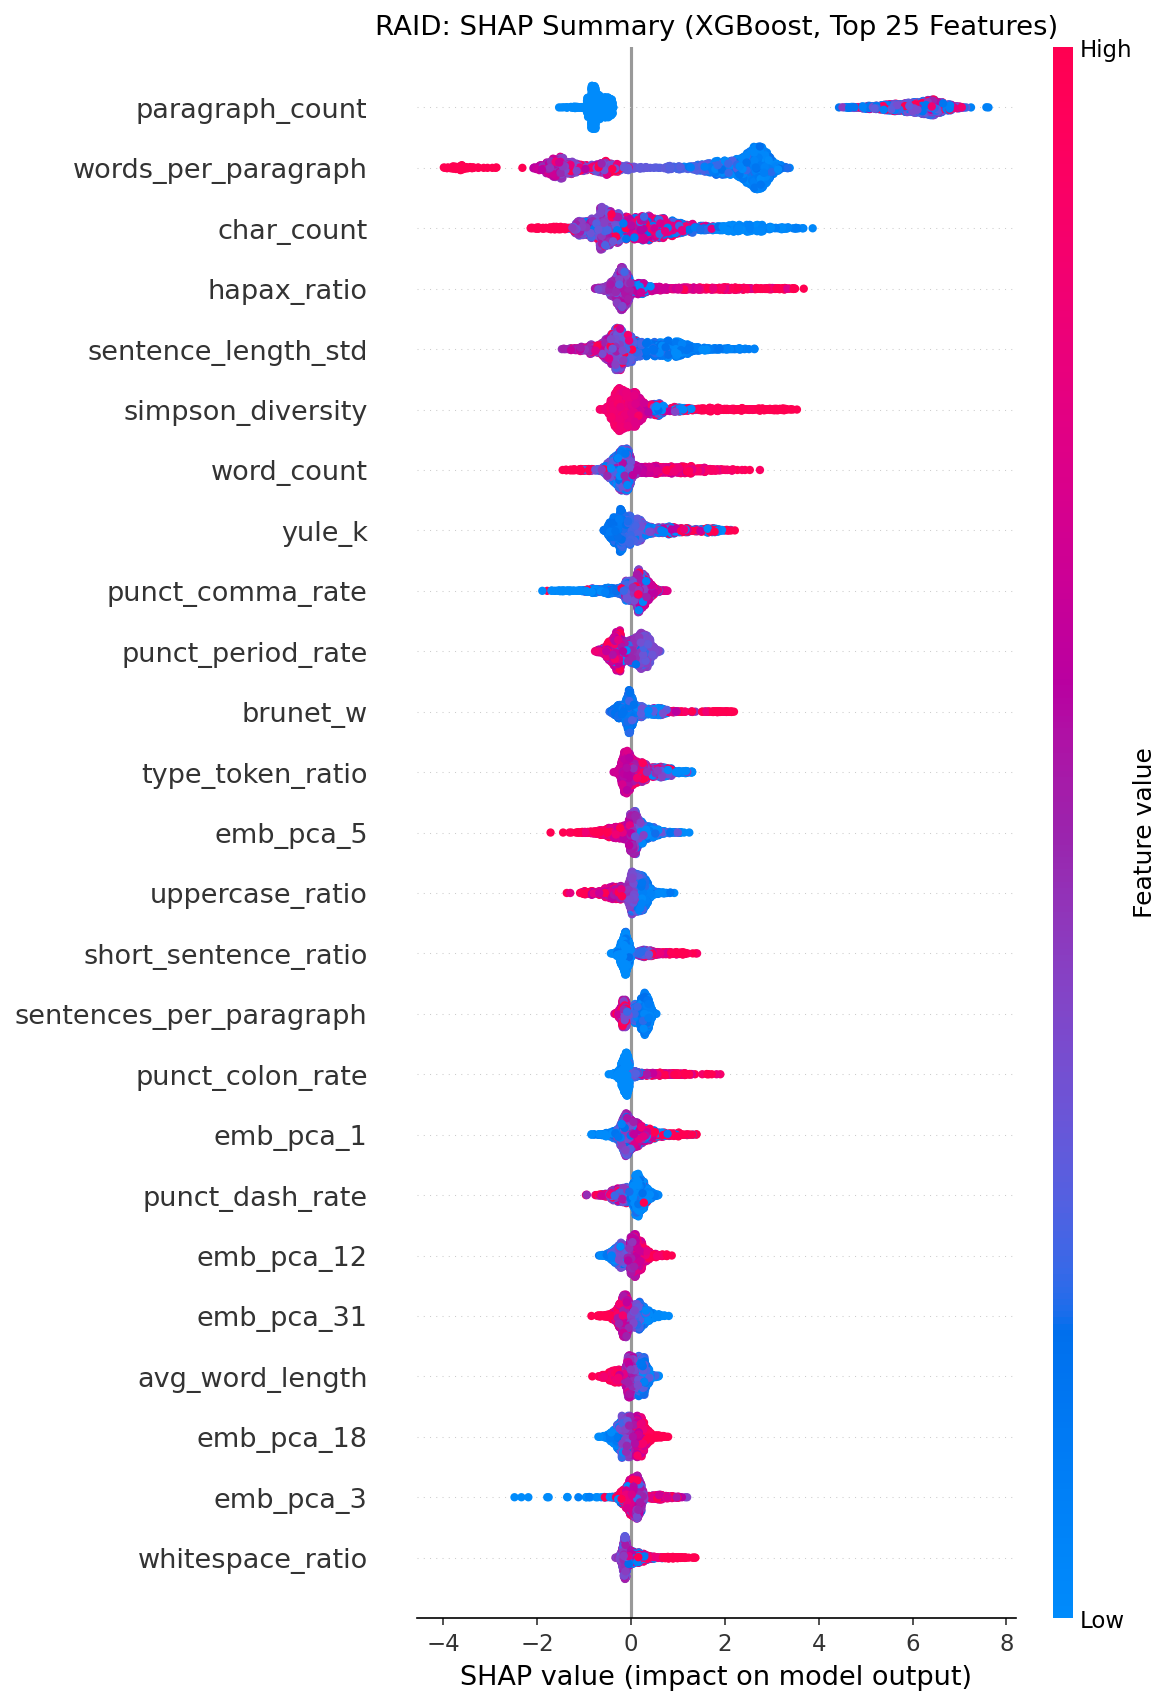
\includegraphics[width=\linewidth]{../figures/raid_shap_summary.png}
    \caption{SHAP feature importance on RAID (top 25 features). Paragraph structure features dominate.}
    \label{fig:shap}
\end{figure}

Figure~\ref{fig:shap} shows the SHAP summary plot. The top features are:
\begin{enumerate}
    \item \textbf{words\_per\_paragraph}---AI text produces shorter, more uniform paragraphs.
    \item \textbf{sentences\_per\_paragraph}---AI paragraphs contain fewer sentences.
    \item \textbf{paragraph\_count}---AI generates more paragraphs for equivalent content.
    \item \textbf{sentence\_length\_std}---human writing has higher sentence length variation.
\end{enumerate}

This aligns with the well-known ``list-making'' tendency of LLMs, which break content into many short paragraphs with bullet points or numbered lists.

\subsection{Per-Generator and Per-Domain Analysis}

\begin{figure}[t]
    \centering
    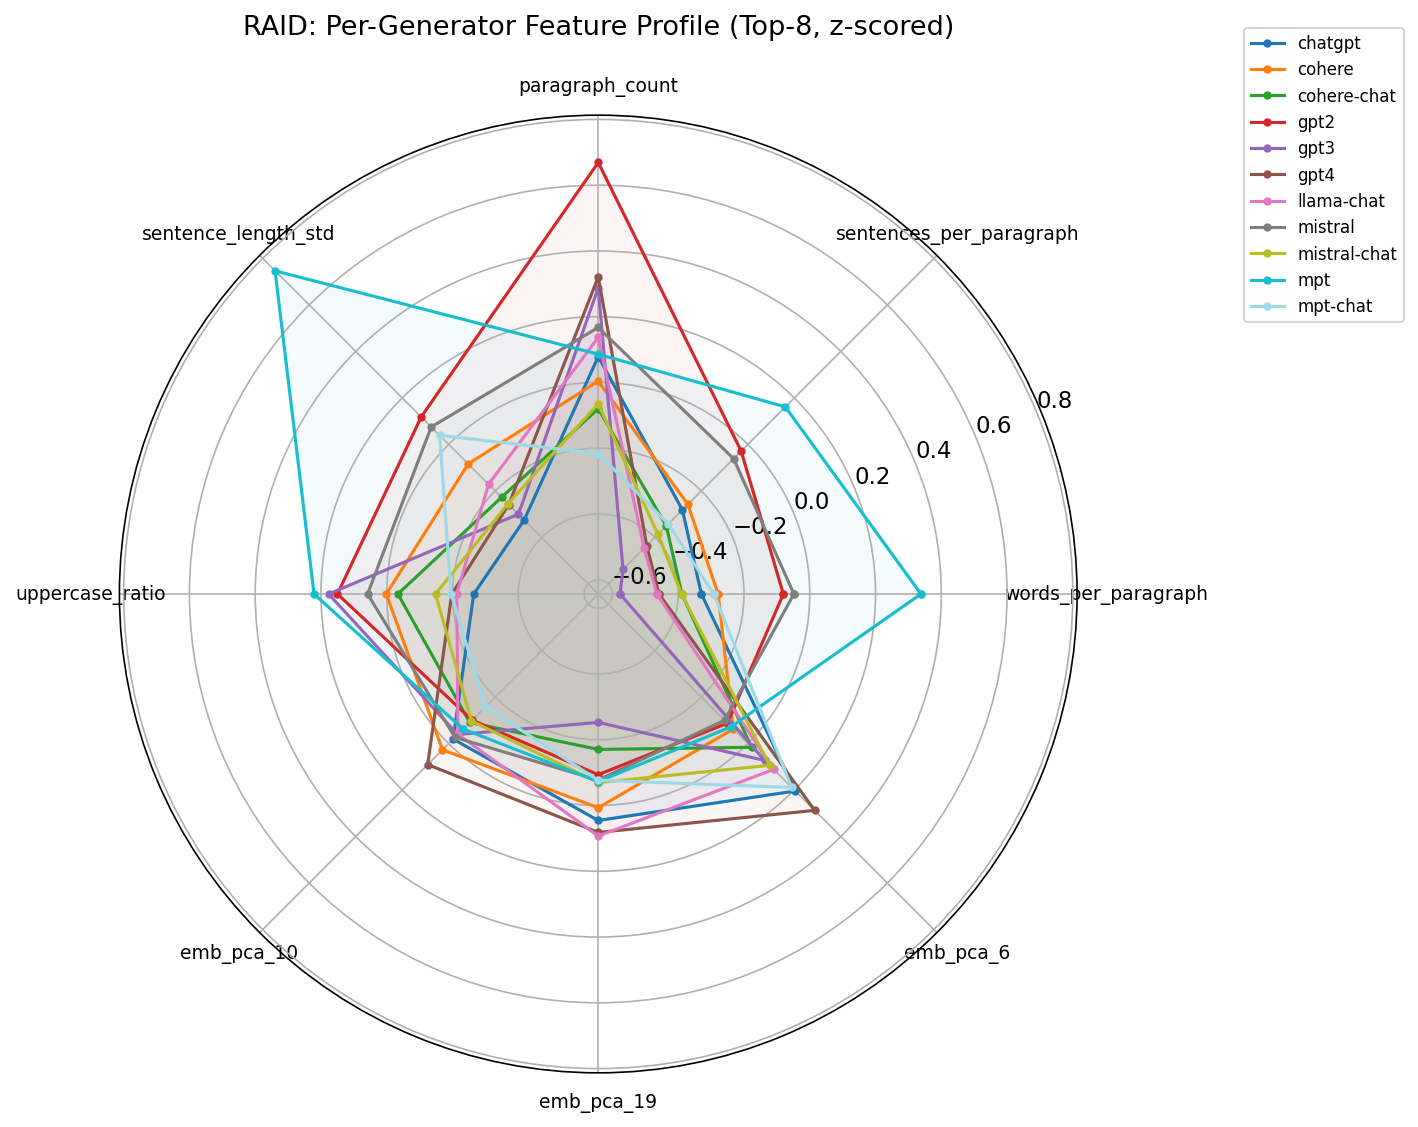
\includegraphics[width=\linewidth]{../figures/raid_generator_radar.png}
    \caption{Per-generator feature profiles (top-8 features, z-scored). Different generators exhibit distinct statistical signatures.}
    \label{fig:radar}
\end{figure}

Figure~\ref{fig:radar} shows per-generator feature profiles. MPT-30B is the hardest to detect (Accuracy 47.4\%), while ChatGPT is easiest (96.2\%). Poetry is the most challenging domain (AUC 0.6137) because human poetry is inherently stylized, reducing the statistical gap.

\subsection{Adversarial Robustness}

\begin{table}[t]
\caption{Adversarial attack robustness (XGBoost, 90 features). Baseline AUC = 0.9951.}
\label{tab:adversarial}
\small
\begin{tabular}{lcc}
\toprule
\textbf{Attack} & \textbf{AUC} & \textbf{Drop} \\
\midrule
insert\_paragraphs       & 0.9915 & $-$0.004 \\
whitespace               & 0.9701 & $-$0.025 \\
synonym                  & 0.9660 & $-$0.029 \\
homoglyph                & 0.9516 & $-$0.044 \\
zero\_width\_space        & 0.8424 & $-$0.153 \\
\textbf{paraphrase}      & \textbf{0.7902} & \textbf{$-$0.205} \\
\bottomrule
\end{tabular}
\end{table}

Table~\ref{tab:adversarial} shows that \textbf{paraphrase attack is the only strategy that significantly degrades detection} (AUC drop 20.5\%). It rewrites the text's lexical and syntactic structure, disrupting most statistical features. Surface-level attacks (spelling, case, number substitution) are almost entirely ineffective, because the majority of our features capture semantic and statistical properties rather than character-level patterns.

\subsection{Cross-Dataset Generalization}

\begin{table}[t]
\caption{Two-layer ablation across 5 datasets (XGBoost AUC). Model-Based sub-groups show distinct effective ranges.}
\label{tab:threelayer}
\small
\begin{tabular}{lccccc}
\toprule
\textbf{Config} & \textbf{RAID} & \textbf{HC3} & \textbf{SemEval} & \textbf{TB} & \textbf{Pile} \\
\midrule
\multicolumn{6}{l}{\textit{Individual layers / sub-groups}} \\
model-free     & 0.994 & 0.995 & 0.517 & 0.670 & 0.962 \\
BERT-emb       & 0.775 & 0.878 & 0.498 & 0.539 & 0.895 \\
GPT2-ppl       & 0.490 & \textbf{0.989} & 0.511 & \textbf{0.975} & 0.504 \\
Mistral-token  & 0.990 & 0.499 & \textbf{0.976} & 0.520 & 0.503 \\
\midrule
\multicolumn{6}{l}{\textit{Combinations}} \\
MB (all)        & 0.994 & 0.994 & 0.961 & 0.970 & 0.894 \\
MF + MB (all)   & \textbf{0.999} & \textbf{1.000} & 0.847 & 0.985 & \textbf{0.973} \\
auto-filter     & \textbf{0.999} & \textbf{1.000} & 0.837 & 0.981 & \textbf{0.973} \\
\bottomrule
\end{tabular}
\end{table}

Table~\ref{tab:threelayer} reveals the core finding: \textbf{each model-based sub-group has a distinct effective range}. GPT-2 perplexity excels on GPT-family text (HC3=0.989, TuringBench=0.975) but fails on diverse generators (RAID=0.490). Mistral-7B token features work on contemporaneous AI (SemEval=0.976) but fail on older generators (TuringBench=0.520). BERT embeddings provide moderate but stable signal across most datasets.

Crucially, na\"{i}vely combining all features can \emph{hurt}: on SemEval, model-based alone (0.961) outperforms MF+MB (0.847) because model-free features are pure noise on this dataset, diluting XGBoost's attention from the informative model-based features.

%% ============================================================
\section{Discussion}

\subsection{Feature Shelf Life and Noise Dilution}

Our two-layer ablation reveals that detection features have ``shelf lives'' tied to the AI generation era. Model-free features were effective against GPT-2/3 era models but have expired for GPT-4/Claude. Within model-based features, each reference model captures a different generation era. This finding has important implications: a production system must \textbf{dynamically assess which sub-groups are informative} for the current detection target.

The noise dilution phenomenon (SemEval: token-only 0.976 $\rightarrow$ all 0.847) occurs because XGBoost allocates importance to uninformative features that happen to correlate with labels in training data. Our Auto-Filter mechanism addresses this by dropping groups with near-random signal strength before training.

\subsection{Practical Deployment Recommendations}

\begin{enumerate}
    \item Use the \textbf{three-layer taxonomy} and assess each layer's signal strength on the target domain before deployment.
    \item Apply \textbf{Auto-Filter} (group-level AUC thresholding) to prevent noise dilution.
    \item \textbf{Update the observer model} periodically (every 6 months) as new generators emerge.
    \item Implement \textbf{paraphrase-specific defenses} as the only effective evasion strategy.
\end{enumerate}

\subsection{Limitations}

Our study has several limitations: (1)~the 90-feature pipeline requires GPT-2 and BERT inference, adding computational overhead; (2)~adversarial analysis is limited to the attacks provided by RAID; (3)~the study does not evaluate on non-English text; (4)~as LLMs continue to improve, the statistical gap between human and AI text may narrow further.

%% ============================================================
\section{Conclusion}

We presented a two-layer interpretable feature taxonomy for AI-generated text detection: model-free statistical features and model-based features from three reference models (118 dimensions total). Through systematic evaluation on RAID and four additional datasets, we demonstrated that:

\begin{enumerate}
    \item \textbf{The two-layer framework achieves AUC 0.9992 on RAID}, rivaling black-box approaches while providing full SHAP-based explainability.
    \item \textbf{Each model-based sub-group has a distinct ``shelf life''}: BERT embeddings capture broad semantic patterns, GPT-2 perplexity is GPT-family-specific, and Mistral-7B token features require temporal alignment.
    \item \textbf{Na\"{i}ve combination can hurt performance} due to noise dilution; our Auto-Filter mechanism addresses this by detecting and discarding uninformative feature groups.
\end{enumerate}

Future work should explore multilingual detection, multi-observer model ensembles, and semantic-level defenses against paraphrase attacks.

%% ============================================================
\bibliographystyle{ACM-Reference-Format}
\begin{thebibliography}{7}

\bibitem{bao2024fast}
Guangsheng Bao, Yanbin Zhao, Zhiyang Teng, Linyi Yang, and Yue Zhang. 2024.
\newblock Fast-DetectGPT: Efficient Zero-Shot Detection of Machine-Generated Text via Conditional Probability Curvature.
\newblock In \emph{ICLR 2024}.

\bibitem{dugan2024raid}
Liam Dugan, Alyssa Hwang, Filip Trhl\'{i}k, Faisal Ladhak, Daphne Ippolito, Chris Callison-Burch, and Eun Jee Lee. 2024.
\newblock RAID: A Shared Benchmark for Robust Evaluation of Machine-Generated Text Detectors.
\newblock In \emph{ACL 2024}.

\bibitem{gao2023hc3}
Chaoqun Gao et al. 2023.
\newblock Human ChatGPT Comparison Corpus (HC3).
\newblock \emph{arXiv:2301.07597}.

\bibitem{gehrmann2019gltr}
Sebastian Gehrmann, Hendrik Strobelt, and Alexander~M. Rush. 2019.
\newblock GLTR: Statistical Detection and Visualization of Generated Text.
\newblock In \emph{ACL 2019}.

\bibitem{hans2024binoculars}
Abhimanyu Hans, Avi Schwarzschild, Valeriia Cheeseman, Carolyn~B. Bruss, and Micah Goldblum. 2024.
\newblock Binoculars: Zero-Shot Detection of LLM-Generated Text.
\newblock In \emph{ICML 2024}.

\bibitem{lundberg2017shap}
Scott~M. Lundberg and Su-In Lee. 2017.
\newblock A Unified Approach to Interpreting Model Predictions.
\newblock In \emph{NeurIPS 2017}.

\bibitem{mitchell2023detectgpt}
Eric Mitchell, Yoonho Lee, Alexander Khazatsky, Christopher~D. Manning, and Chelsea Finn. 2023.
\newblock DetectGPT: Zero-Shot Machine-Generated Text Detection using Probability Curvature.
\newblock In \emph{ICML 2023}.

\end{thebibliography}

\end{document}
